\section{Update}\label{model-update}
This section describes one approach for reliable model updates.
The updater assumes that it is given a sample of data $S_{dirty}$ from $R_{dirty}$ where $i \in S_{dirty}$ has a known sampling probability $p(i)$.
The following sections show how to optimize $p(i)$ and the analysis in this section applies for any sampling distribution $p(\cdot)$.

\subsection{Geometric Derivation}
The update algorithm intuitively follows from the convex geometry of the problem.
Consider this problem in one dimension (i.e., the parameter $\theta$ is a scalar value), so then the goal is to find the minimum point ($\theta$) of a curve $l(\theta)$.
The consequence of dirty data is that the the wrong loss function is optimized.
Figure \ref{update-arch2}A illustrates the consequence of this optimization.
The red dotted line shows the loss function on the dirty data.
Optimizing this loss function finds $\theta$ that at the minimum point (red star).
However, the true loss function (w.r.t to the clean data) is in blue, thus
this optimal value on the dirty data is in fact a suboptimal point on clean curve (red circle).

\begin{figure}[ht!]
\centering
 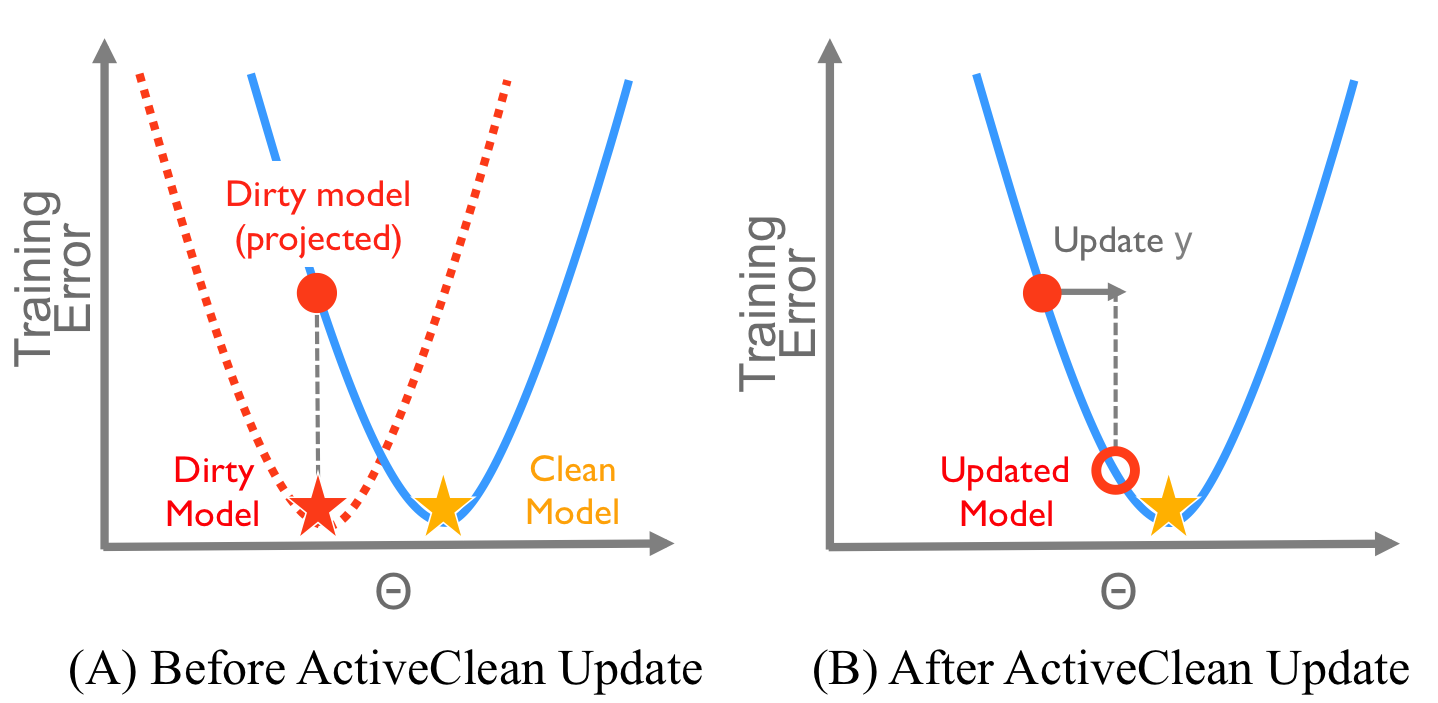
\includegraphics[width=\columnwidth]{figs/update-arch2.png}\vspace{-1em}
 \caption{(A) A model trained on dirty data can be thought of as a sub-optimal point w.r.t to the clean data. (B) The gradient gives us the direction to move the suboptimal model to approach the true optimum. \label{update-arch2}}\vspace{-1em}
\end{figure}

The optimal clean model $\theta^{(c)}$ is visualized as a yellow star.
The first question is which direction to update $\theta$ (i.e., left or right).
For this class of models, given a suboptimal point, the direction to 
the global optimum is the gradient of the loss function.
The gradient is a $d$-dimensional vector function of the current model $\theta$ and the clean data.
Given this direction, \sys needs to update $\theta^{(d)}$ some distance $\gamma$ (Figure \ref{update-arch2}B):
\[
\theta^{new} \leftarrow \theta^{(d)} - \gamma \cdot \nabla\phi(\theta^{(d)})
\]
At the optimal point, the magnitude of the gradient will be zero.
So intuitively, this approach iteratively moves the model downhill (transparent red circle) -- correcting the dirty model until the desired accuracy is reached.
However, this formulation gradient depends on all of the clean data which is not available and \sys will have to approximate this gradient from a sample.
The main intuition is that if the gradient steps are on average correct, the model still moves downhill albeit with a reduced convergence rate proportional to the inaccuracy of the sample-based estimate.

To derive a sample-based update rule, the most important property is that sums commute with derivatives and gradients.
The convex loss class of models are sums of losses, so given the current best model $\theta$, the gradient $g^*(\theta)$ is:
\[
g^*(\theta) = \nabla\phi(\theta) = \frac{1}{N} \sum_i^N \nabla\phi(x_i^{(c)},y_i^{(c)},\theta)
\]
\sys needs to estimate $g^*(\theta)$ from a sample $S$ is drawn from the dirty data $R_{dirty}$ so this sum has two components the gradient on the already clean data $g_C$ which can be computed without cleaning and $g_S$ the gradient estimate from a sample of dirty data to be cleaned:
\[
g(\theta) = \frac{\mid R_{clean} \mid}{\mid R \mid} \cdot g_C(\theta) + \frac{\mid R_{dirty} \mid}{\mid R \mid} \cdot g_S(\theta)
\]
$g_C$ can be calculated by applying the gradient to all of the already cleaned records:
\[
g_C(\theta) = \frac{1}{\mid R - R_{dirty}\mid}\sum_{i \in R - R_{dirty}}\nabla\phi(x_i^{(c)},y_i^{(c)},\theta)
\]
$g_S$ can be estimated from a sample by taking the gradient w.r.t each record, and re-weighting the average by their respective sampling probabilities.
Before taking the gradient the cleaning function $C(\cdot)$ is applied to each sampled record.
Therefore, let $S$ be a sample of data, where each $i \in S$ is drawn with probability $p(i)$:
\[
g_{S}(\theta) = \frac{1}{\mid S \mid} \sum_{i \in S}\frac{1}{p(i)}\nabla\phi(x_i^{(c)},y_i^{(c)},\theta)
\]
Then, at each iteration $t$, the update becomes:
\[
\theta^{(t+1)} \leftarrow \theta^{(t)} - \gamma \cdot g(\theta^{(t)})
\]

\subsection{Model Update Algorithm}
To summarize, the algorithm is initialized with $\theta^{(1)} = \theta^{(d)}$ which is the dirty model.
There are three user set parameters the budget $k$, batch size $b$, and the step size $\gamma$.
In the following section, we will provide references from the convex optimization literature that allow the user to appropriately select these values.
At each iteration $t=\{1,...,T\}$, the cleaning is applied to a batch of data $b$ selected from the set of candidate dirty records $R_{dirty}$.
Then, an average gradient is estimated from the cleaned batch and the model is updated.
Iterations continue until $k = T \cdot b$ records are cleaned.

\begin{enumerate}[noitemsep]
	\item Calculate the gradient over the sample of clean data and call the result $g_S(\theta^{(t)})$
	\item Calculate the average gradient over all the data in $R_{clean}=R-R_{dirty}$, and call the result $g_C(\theta^{(t)})$
	\item Apply the following update rule:
	\[
	\theta^{(t+1)} \leftarrow \theta^{(t)} - \gamma \cdot(\frac{\mid R_{dirty} \mid}{\mid R \mid} \cdot g_S(\theta^{(t)}) + \frac{\mid R_{clean} \mid}{\mid R \mid} \cdot  g_C(\theta^{(t)}))
	\]
\end{enumerate} 

\subsection{Analysis with Stochastic Gradient Descent}\label{sgd}
This update policy can be formalized as a class of very well studied algorithms called Stochastic Gradient Descent.
This provides a theoretical framework to understand and analyze the update rule and bound the error.
Mini-batch stochastic gradient descent (SGD) is an algorithm for finding the optimal value
given the convex loss and data.
In mini-batch SGD, random subsets of data are selected at each iteration and the average gradient is computed for every batch.

One key difference with traditional SGD models is that \sys applies a \emph{full} gradient step on the already clean data and averages this with a stochastic gradient step (i.e., calculated from a sample) on the dirty data. 
Therefore, \sys iterations can take multiple passes over the clean data but at most a single cleaning pass of the dirty data.
This update method can be thought of as a variant of SGD that lazily materializes the clean value.
As data is sampled at each iteration, data is cleaned when needed by the optimization.
It is well known that even for an arbitrary initialization SGD makes significant progress in less than one epoch (a pass through the entire dataset) \cite{bottou2012stochastic}.
In practice, the dirty model can be much more accurate than an arbitrary initialization as corruption may only affect a few features and combined with the full gradient step on the clean data the updates coverge very quickly.

\vspace{0.25em}

\noindent\textbf{ Setting the step size $\gamma$: } There is extensive literature in machine learning for choosing the step size $\gamma$ appropriately. $\gamma$ can be set either to be a constant or decayed over time. Many machine learning frameworks (e.g., MLLib, Sci-kit Learn, Vowpal Wabbit) automatically set learning rates or provide different learning scheduling frameworks. 
In the experiments, we use a technique called inverse scaling where there is a parameter $\gamma_0=0.1$, and at each iteration it decays to $\gamma_t = \frac{\gamma_0}{\mid S \mid t}$. 

\vspace{0.25em}

\noindent\textbf{ Setting the batch size: } The batch size should be set by the user to have the desired properties.
Larger batches will take longer to clean and will make more progress towards the clean model, but will have less frequent model updates.
On the other hand, smaller batches are cleaned faster and have more frequent model updates but make less progress.
The overheads introduced by \sys are more evident at smaller batch sizes.
There are diminishing returns to increasing the batch size $O(\frac{1}{\sqrt{b}})$.
Empirically, in the experiments, batch sizes of 50 converge the fastest.
If a data cleaning technique requires a larger batch size than this, i.e., data cleaning is fast enough that the iteration overhead is significant compared to cleaning 50 records, \sys can apply the updates in smaller batches.
For example, the batch size set by the user might be $b=1000$, but the model updates after every $50$ records are cleaned.
This dissociates the batching requirements of SGD and the batching requirements of the data cleaning technique.

\subsubsection{Convergence Conditions and Properties}
Convergence properties of batch SGD formulations have been well studied \cite{dekel2012optimal}.Essentially, if the gradient estimate is unbiased and the step size is appropriately chosen, the algorithm is guaranteed to converge. 
In the appendix, we show that the gradient estimate from \sys is indeed unbiased and our choice of step size is one that is established to converge.
The convergence rates of SGD are also well analyzed \cite{dekel2012optimal,bertsekas2011incremental,zhao2014stochastic}. 
This gives a bound on the error of intermediate models and the expected number of steps before achieving a model within a certain error. 
For a general convex loss, a batch size $b$, and $T$ iterations, the convergence rate is bounded by $O(\frac{\sigma^2}{\sqrt{bT}})$. 
$\sigma^2$ is the variance in the estimate of the gradient at each iteration:
\[
\mathbb{E}(\|g_S - g^*\|^2)
\]
If the loss in non-convex, the update procedure will converge towards a local minimum rather than the global minimum (See Appendix \ref{non-convex}).

\subsection{Example}
This example describes an application of the update algorithm.
\begin{example}\label{upex}
Recall that the analyst has a dirty SVM model on the dirty data $\theta^{(d)}$.
She decides that she has a budget of cleaning $100$ records, and decides to clean the 100 records in batches of 10 (set based on how fast she can clean the data, and how often she wants to see an updated result).
All of the data is initially treated as dirty with $R_{dirty} = R$ and $R_{clean} = \emptyset$.
The gradient of a basic SVM is given by the following function:
\[
\nabla\phi(x,y,\theta) =
\begin{cases}      
-y\cdot\boldsymbol{x} \text{ if } y\cdot\boldsymbol{x}\cdot\theta \le 1 \\
0\ \text{ if } y\ \boldsymbol{x}\cdot\theta \geq 1      
\end{cases}
\]

For each iteration $t$, a sample of 10 records $S$ is drawn from $R_{dirty}$.
\sys then applies the cleaning function to the sample:
\[
\{(x_i^{(c)},y_i^{(c)})\} = \{C(i): \forall i \in S\}
\]
Using these values, \sys estimates the gradient on the newly cleaned data:
\[
g_{S}(\theta) = \frac{1}{10} \sum_{i \in S}\frac{1}{p(i)}\nabla\phi(x_i^{(c)},y_i^{(c)},\theta)
\]
\sys also applies this gradient to the already clean data (initially non-existent):
\[
g_C(\theta) = \frac{1}{\mid R_{clean}\mid}\sum_{i \in R - R_{dirty}}\nabla\phi(x_i^{(c)},y_i^{(c)},\theta)
\]
Then, it calculates the update rule:
\[
	\theta^{(t+1)} \leftarrow \theta^{(t)} - \gamma \cdot(\frac{\mid R_{dirty} \mid}{\mid R \mid} \cdot g_S(\theta^{(t)}) + \frac{\mid R_{clean} \mid}{\mid R \mid} \cdot  g_C(\theta^{(t)}))
\] 
Finally, $R_{dirty} \leftarrow R_{dirty} - S$, $R_{clean} \leftarrow R_{clean} + S$, and continue to the next iteration.
\end{example}
